% !TEX root =  tb_icml_2018.tex

\section{Introduction}
\label{sec:intro}
Variational bounds provide tractable and state-of-the-art objectives for training deep generative models \citep{kingma2014auto,rezende2014stochastic}.  Typically taking
the form of a lower bound on the intractable model evidence, 
they provide surrogate targets that are more amenable to optimization.
%with this optimization typically carried out using a variant of \gls{SGA}~\citep{robbins1951stochastic,kingma2014adam}.
In general, this optimization
%typically carried out using a variant of \gls{SGA}~\citep{robbins1951stochastic,kingma2014adam},
requires the generation of approximate posterior samples during the model
training and so a number of methods simultaneously learn an \emph{inference
network} alongside the target \emph{generative network}. 

As well as assisting the training process, this inference network is often also of
direct interest itself.  For example, variational bounds are often used to train 
auto-encoders~\citep{bourlard1988auto,hinton1994autoencoders,gregor2016towards,chen2016variational},
for which the inference network forms the encoder.
Variational bounds are also used in amortized and traditional Bayesian inference 
 contexts~\cite{hoffman2013stochastic,ranganath2014black,
 	paige2016inference,le2017inference}, for which the generative model
 is fixed and the inference network is the primary target for the training.

The performance of variational approaches depends upon the choice of
evidence lower bound (\gls{ELBO})
and the formulation of the inference network, with the two often intricately linked to one another;
if the inference network formulation is not sufficiently expressive, this can have 
a knock-on effect on the generative network~\citep{burda2016importance}.  
In choosing the \gls{ELBO}, it is often implicitly
assumed that using tighter \glspl{ELBO} is universally beneficial,
at least whenever this does not in turn lead to higher variance 
gradient estimates.


% and
%that larger values of the \gls{ELBO} indicate
%a better model.  
In this work we question this implicit assumption
by demonstrating that,
although using a tighter \gls{ELBO} is typically beneficial to gradient 
%\begin{wrapfigure}{r}{0.26\textwidth}
%	\centering
%		\vspace{-7pt}
%	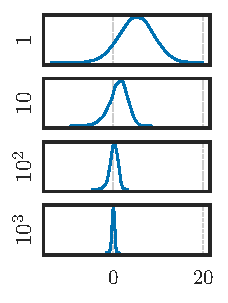
\includegraphics[width=0.24\textwidth]{gaussian_gradient.pdf}
%	\vspace{-15pt}
%	\caption{Density of $\nabla_{\phi} \ELBO$ 
%		for different $K$.}
%	\label{fig:kde}
%	\vspace{-20pt}
%\end{wrapfigure}
updates of the 
generative network, it can be detrimental to updates of
 the inference network.
Remarkably, we find that it is possible to simultaneously tighten the bound,
reduce the variance of the gradient updates, and \emph{arbitrarily deteriorate} the
training of the inference network.

Specifically, we present theoretical and empirical evidence that increasing the
number of importance sampling particles, $K$, to tighten the bound in the \gls{IWAE}~\citep{burda2016importance}, degrades the \gls{SNR} of the
gradient estimates for the inference network, inevitably deteriorating the overall learning process.  In short, this behavior manifests because even though increasing
$K$ decreases the standard deviation of the gradient estimates, it decreases
the magnitude of the true gradient faster, such that the \emph{relative variance increases}.
%
%An intuitive demonstration of this effect is given in Figure~\ref{fig:kde}.
%This shows a kernel density estimation for the distribution of the \gls{ELBO} gradient
%estimator with respect to the proposal parameter $A$ for the model discussed in 
%Section~\ref{sec:emp} (with $D=N=1$) and different $K$.
%We see that as we increase $K$, both the amplitude of the gradient
%and the standard deviation of the estimator decrease.
%However, because the former reduces faster, the \gls{SNR} deteriorates.
%This is perhaps easiest
%to appreciate by noting that for the larger values of $K$, there is a roughly equal probability
%of the estimator being positive or negative, such that we are equally likely to increase or decrease
%the parameter value at the next iteration, inevitably leading to poor performance.
%On the other hand, when $K=1$, it is far more likely that the gradient estimator is positive
%than negative and so there is clear drift to the gradient steps.
%Note that using a larger
%$K$ should always give better performance at test time~\citep{cremer2017reinterpreting}
% -- the implication of our
%result is that it may be better to learn the inference network using a smaller $K$ during
%training.

Our results suggest that it may be best to use distinct objectives for learning
the generative and inference networks, or that when using the same target, it should
take into account the needs of both networks.
%As a consequence of these results, we assert that it is not, in general, best to use the
%same objective for learning the generative and inference networks. 
Namely, while tighter bounds are typically better for training
the generative network, looser bounds often lead to better
training of the inference network.
Based on these insights, we introduce three new algorithms: the \gls{PIWAE}, the \gls{MIWAE}, and the \gls{CIWAE}. Each of these include \gls{IWAE} as a special case and are based on the same set of importance weights, 
but use these weights in different ways to ensure a higher SNR for the
inference network.  

We demonstrate that
our new algorithms can produce inference networks more closely representing the true posterior
than~\gls{IWAE}, while matching the
training of the generative network, or potentially even improving it in the case of~\gls{PIWAE}. 
Even when treating the \gls{IWAE} 
objective itself as the measure of performance, all our algorithms are able to demonstrate clear
improvements over \gls{IWAE}.

%
%We therefore propose  the \gls{PIWAE} which uses the
%\gls{IWAE} objective for updating the generative network parameters, but the looser
%\gls{VAE} objective (estimated using the same $K$ samples) to update the inference
%network.  By using a target for the inference network with a higher \gls{SNR}, the
%\gls{PIWAE} provides more effective updates for the inference network, without degrading
%those of the generative network.  We demonstrate that, over multiple iterations,
%this leads to improved training of both networks, and ultimately improved models and 
%amortized inference schemes.

\section{Background and Notation}

Let $x$ be an $\mathcal{X}$-valued random variable defined via a process involving an unobserved $\mathcal{Z}$-valued random variable $z$ with joint density $p_{\theta}(x, z)$. Direct maximum likelihood estimation of $\theta$ is generally intractable if  $p_{\theta}(x, z)$ is a deep generative model due to the marginalization of $z$. A common strategy is to instead optimize a variational lower bound on $\log p_{\theta}(x)$, defined via an auxiliary inference model $q_{\phi}(z \given x)$:
\begin{align}
	\ELBO_{\text{VAE}} &(\theta, \phi, x) \coloneqq \int q_{\phi}(z \given x) \log \frac{p_{\theta}(x, z)} {q_{\phi}(z \given x)} \,\mathrm dz \nonumber \\
	&= \log p_{\theta}(x) - \mathrm{KL}(q_{\phi}(z \given x) || p_{\theta}(z \given x)). \label{eqn:intro/elbo_vae}
\end{align}
Typically, $q_{\phi}$ is parameterized by a neural network, for which the approach is known as the \gls{VAE}~\citep{kingma2014auto,rezende2014stochastic}. Optimization
is performed with \gls{SGA} using unbiased estimates of $\nabla_{\theta, \phi} \ELBO_{\text{VAE}}(\theta, \phi, x)$. If $q_{\phi}$ is reparameterizable, %~\citep{kingma2014auto, rezende2014stochastic},
% then given a sample  $z \sim q_{\phi}(z  \given x)$, the gradients $\nabla_{\theta, \phi} \left(\log p_{\theta}(x, z) - \log q_{\phi}(z \given x)\right)$ can be used for optimization, taking care to note that,  in general, $\nabla_{\phi} z \neq 0$ due to
% the reparameterization.
then given a reparameterized sample  $z \sim q_{\phi}(z  \given x)$, the gradients $\nabla_{\theta, \phi} (\log p_{\theta}(x, z) - \log q_{\phi}(z \given x))$ can be used for the 
optimization.

The \gls{VAE} objective places a harsh penalty on mismatch between $q_{\phi}(z \given x)$ and $p_{\theta}(z \given x)$; optimizing jointly in $\theta, \phi$ can confound improvements in $\log p_{\theta}(x)$ with reductions in the KL \citep{turner2011two}. Thus, research has looked to develop bounds that separate the tightness of the bound from the expressiveness of the class of $q_{\phi}$. For example, the \gls{IWAE} objectives~\citep{burda2016importance}, which we
denote as $\ELBO_{\text{IS}}(\theta, \phi, x)$, are a family of bounds defined by
\begin{align}
	Q_{\text{IS}}(z_{1:K} \given x) &\coloneqq \prod\nolimits_{k = 1}^K q_{\phi}(z_k \given x), \nonumber
	\\
	\hat Z_{\text{IS}}(z_{1:K}, x) &\coloneqq \frac{1}{K}\sum\nolimits_{k = 1}^K \frac{p_{\theta}(x, z_k)}{q_{\phi}(z_k \given x)}, \label{eq:background/q_is_z_is}\\
	\ELBO_{\text{IS}}(\theta, \phi, x) &\coloneqq \int Q_{\text{IS}}(z_{1:K} \given x) \log \hat Z_{\text{IS}}(z_{1:K}, x) \,\mathrm dz_{1:K}
	% \leq \log \int Q_{\text{IS}}(x^{1:K}) \hat Z_{\text{IS}}(x^{1:K}) \,\mathrm dx^{1:K}
	% = \log p_{\theta}(x), \label{eq:background/elbo-is} \\
	\nonumber
 %\label{eq:background/elbo-is}
\end{align}
$\leq \log p_{\theta}(x)$.
The \gls{IWAE} objectives generalize the \gls{VAE} objective ($K=1$ corresponds to the \gls{VAE}) and the bounds become strictly tighter as $K$ increases \cite{burda2016importance}. When the family of $q_{\phi}$ contains the true posteriors, the global optimum parameters $\{\theta^*,\phi^*\}$ are independent of $K$, see e.g.~\cite{le2017auto}. Nonetheless, except for the most trivial models, it is not usually the case that $q_{\phi}$ contains the true posteriors, and \citet{burda2016importance} provide strong empirical evidence that setting
$K>1$ leads to significant empirical gains over the \gls{VAE} in terms of learning the
generative model. 

Optimizing tighter bounds is usually empirically associated with 
better models $p_{\theta}$ in 
terms of marginal likelihood on held out data.
Other related approaches extend this to \gls{SMC} \citep{maddison2017filtering, le2017auto,naesseth2017variational} or change the lower bound that is optimized to reduce the bias \citep{li2016renyi,bamler2017perturbative}.
A second, unrelated, approach is to tighten the bound by improving the expressiveness of $q_{\phi}$ \citep{salimans_markov_2015, tran_variational_2015, rezende_variational_2015, kingma2016improving, maaloe_auxiliary_2016, ranganath2016hierarchical}.
In this work, we focus on the former, algorithmic, approaches to tightening bounds. 

%We present theoretical and empirical evidence that increasing $K$ makes $\ELBO_{\text{IS}}(\theta, \phi, x)$ 
%a worse objective from the perspective of learning $q_{\phi}$. In particular, as $K$ increases, the learned $q_{\phi}$ becomes a worse approximation of the posterior $p_{\theta}(z|x)$ with which it is jointly learnt. This result is perhaps somewhat counter intuitive: it directly implies that
%reducing the variance of the marginal likelihood estimate $\hat Z_{\text{IS}}(z^{1:K}, x)$
%worsens the estimates for $\nabla_{\phi} \ELBO_{\text{IS}}(\theta, \phi, x)$.  We emphasise
%that this is degradation in performance as the computational effort expended is increased,
%not just a relative decrease to using the samples in a different way.
%At a high level, this usual effect arises from the fact that the \gls{SNR} of the
%reparameterization gradients of $\phi$ decreases with $K$ (specifically at a rate $O(1/\sqrt{K})$): though the standard deviation of the estimate decreases, its expected value decreases faster,
%giving a net negative effect on the \gls{SNR}.
%Thus, to the extent that improving the optimization with respect to $\phi$ improves the final model $p_{\theta}$, this implies that improvements in algorithms can be made by optimizing distinct objectives for $q_{\phi}$ and $p_{\theta}$.  We exploit this insight by introducing \gls{PIWAE},
%which still targets $\ELBO_{\text{IS}}(\theta, \phi, x)$  for optimization of the generative network
%parameters $\theta$, but instead targets $\ELBO_{\text{VAE}}(\theta, \phi, x)$ for
%optimization of the inference network parameters $\phi$.

%
%\begin{itemize}
%\item If we want to diminish the effect of single bad samples, we should probably just
%downscale the KL divergence rather than using a lower bound as this maintains
%the signal-to-noise ratio.
%\item The IWAE argument that its bad to let a few bad samples cause harsh penalization
%is highly dubious.  They are effectively arguing for softening the target gradients --
%a proposal that avoids these is still clearly better so even if we can't achieve it, we want
%this information for our gradient updates.  The question is thus probably more to
%do with the relative trade-off of the log marginal and KL terms, than it is using a proposal
%that lowers the KL.
%\item Using a more powerful proposal form (i.e. multiple samples) during training may
%not always be helpful or beneficial -- using a worse one can force the learning of
%good proposals that then get even better if we use multiple samples at run time.
%\item Still probably help model learning through improving the inference, but we should
%just learn the model and then learn a proposal for this model.
%\end{itemize}